% !TeX root = ../main.tex
\chapter{Unidad 5: Análisis frecuencial de señales acústicas}

\section*{Objetivo pedagógico}
\noindent\textbf{Objetivo.} Comprender cómo las herramientas de Fourier descomponen señales acústicas en sus frecuencias, explorar los rangos de frecuencia y el rango dinámico del oído humano, y aplicar filtros y curvas de ponderación (A, C, Z) en contextos clínicos de fonoaudiología, como el análisis de la voz o la calibración de cabinas audiométricas. Se incluyen ejemplos clínicos, actividades prácticas, recursos multimedia y ejercicios de autoevaluación.

\noindent\textbf{Pregunta inicial.} ¿Cómo puede un fonoaudiólogo analizar la voz de un paciente para detectar problemas? ¿Por qué algunos sonidos son más fáciles de escuchar que otros? ¡Esta unidad te ayudará a entender cómo descomponemos y medimos el sonido!

\section{Herramientas de Fourier}
Las herramientas de Fourier permiten descomponer una señal acústica (como la voz) en sus frecuencias individuales, como separar los colores de un arcoíris.

\subsection{Series de Fourier}
Una serie de Fourier es una representación matemática de una función periódica (con periodo $T$) como una suma infinita de funciones seno y coseno:
\[
x(t) = a_0 + \sum_{n=1}^{\infty} \left[ a_n \cos(2\pi n f t) + b_n \sin(2\pi n f t) \right], \quad f_0 = \frac{1}{T}
\]

La serie de Fourier descompone una función periódica en una suma de funciones senoidales y cosenoidales, cada una con una frecuencia diferente y una amplitud específica. Estas funciones senoidales y cosenoidales se denominan armónicos y la frecuencia más baja es la fundamental.

\begin{figure}[h]
    \centering
    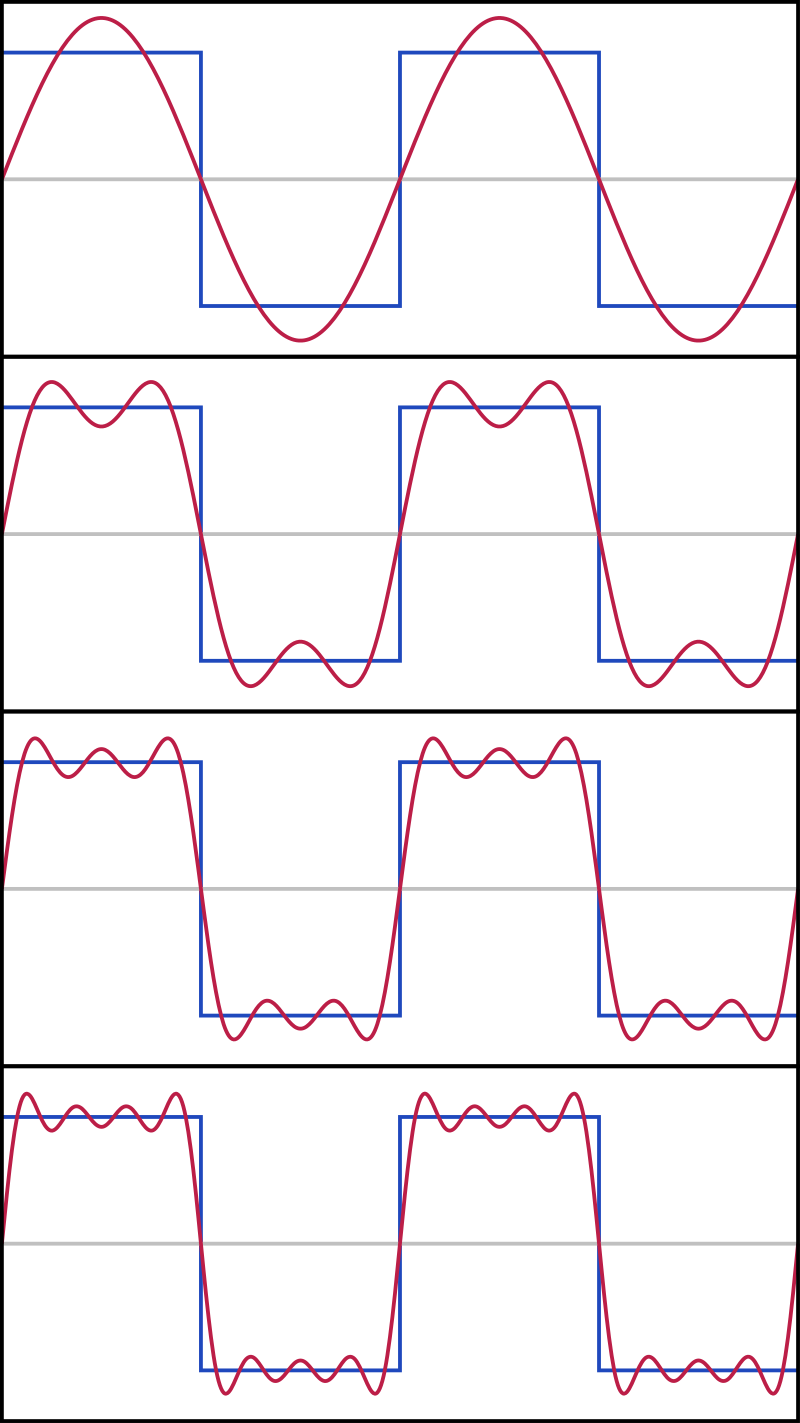
\includegraphics[width=0.4\textwidth]{figures/fourier.png}
    \caption{Aproximación a una función escalonada mediante los primeros 4 armónicos de su serie de Fourier.}
    \label{fourier}
\end{figure}

\begin{quote}
    \textbf{Ejemplo clínico.} La voz humana tiene una frecuencia fundamental ($f_0$, como 120 Hz para un hombre) y armónicos que dan su timbre único, analizados en trastornos como la disfonía.
\end{quote}

\subsection{Transformada de Fourier (FT)}
Para señales no periódicas (como una frase hablada), la transformada de Fourier muestra todas las frecuencias presentes:
\[
X(f) = \int_{-\infty}^{\infty} x(t) e^{-j 2\pi f t} \, dt.
\]
El \textbf{espectro de amplitud} ($|X(f)|$) muestra la intensidad de cada frecuencia. En la práctica, usamos la \textbf{FFT} (Transformada Rápida de Fourier) con ventanas (como Hann) para crear espectrogramas.

\begin{quote}
    \textbf{Ejemplo clínico.} Un espectrograma de la vocal /a/ muestra picos (formantes) que ayudan a diagnosticar problemas de articulación o resonancia.
\end{quote}

\begin{figure}[h]
    \centering
    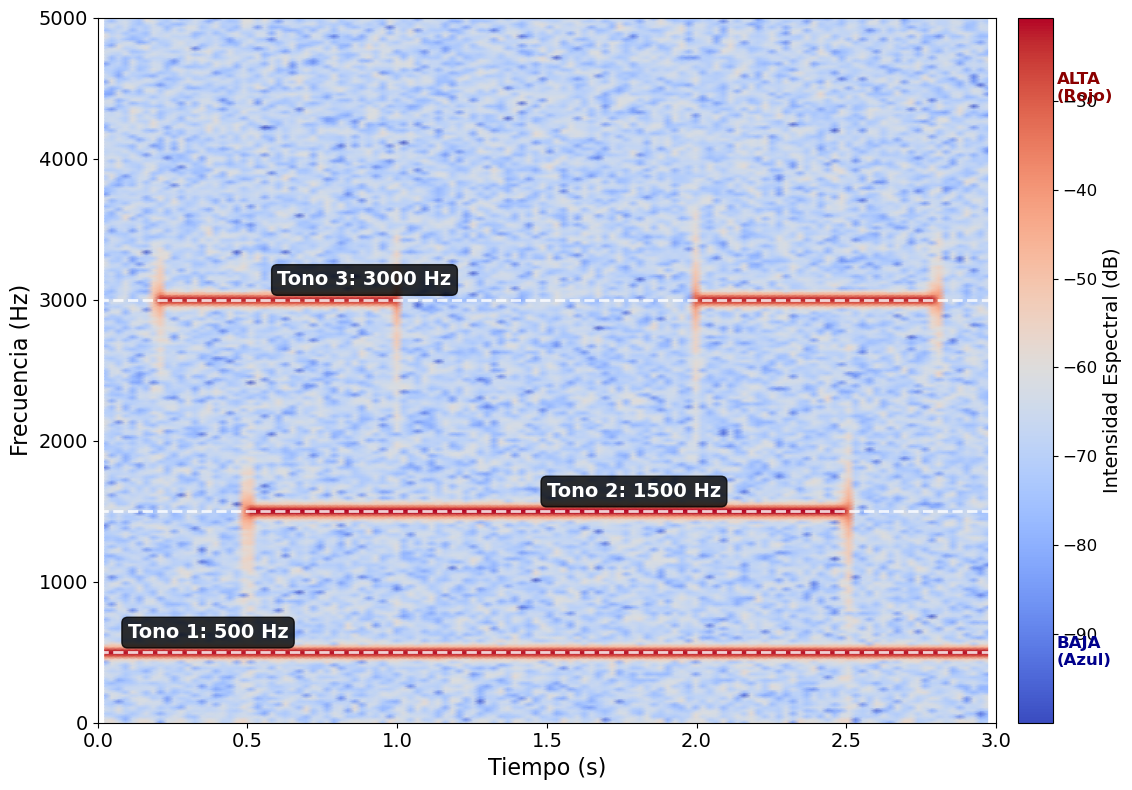
\includegraphics[width=1.0\textwidth]{figures/espectrograma.png}
    \caption{Espectrograma de una función de 3 tonos puros.}
    \label{espectrograma}
\end{figure}

\textbf{Actividad práctica.} Usa Audacity (gratis) para grabar una vocal como /a/. Ve al menú ``Análisis'' → ``Espectro'' y observa los picos de frecuencia (formantes). Compara con una vocal susurrada.

\section{Gráficos de respuesta en frecuencia}
Un gráfico de respuesta en frecuencia muestra la intensidad (en dB) frente a la frecuencia (en Hz). Los picos indican resonancias, como los formantes de la voz (F1, F2, F3), que dan el timbre.

\begin{quote}
    \textbf{Ejemplo clínico.} Un audífono se ajusta según la respuesta en frecuencia del oído del paciente, amplificando frecuencias donde hay pérdida auditiva (por ejemplo, 4000 Hz para presbiacusia).
\end{quote}

\begin{figure}[h]
    \centering
    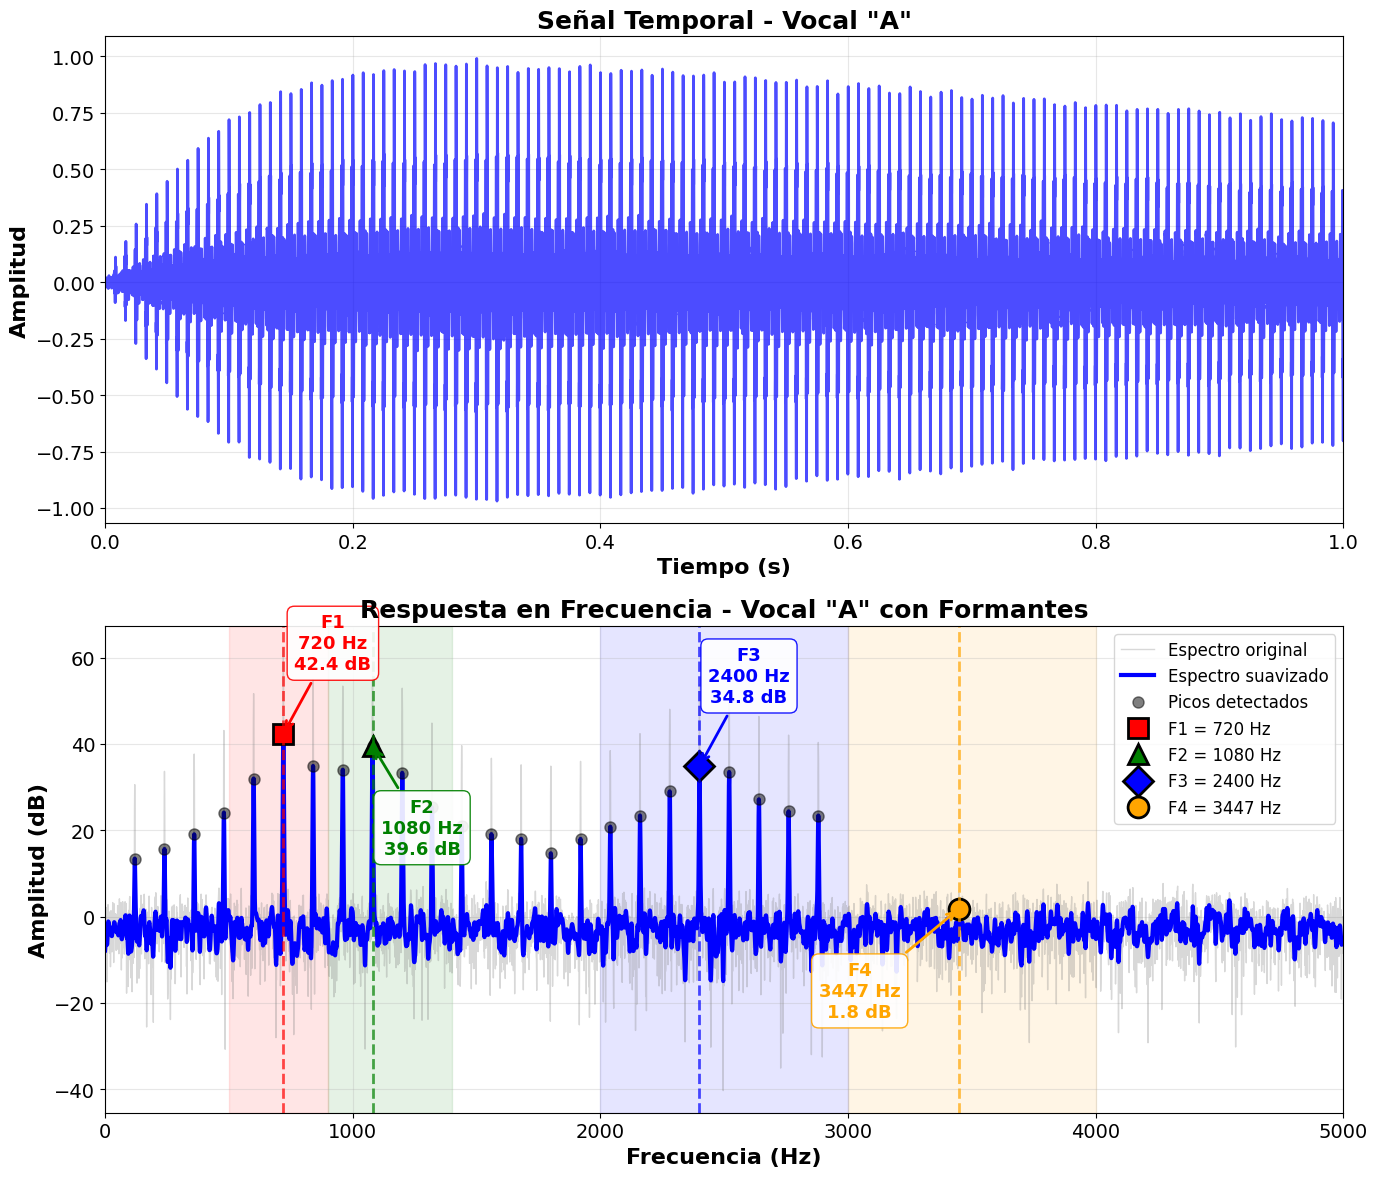
\includegraphics[width=1.0\textwidth]{figures/rta_freq_vocal.png}
    \caption{Gráfico de respuesta en frecuencia para la vocal \textit{/a/} y sus formantes.}
    \label{rta_freq_vocal}
\end{figure}


\section{Rangos de frecuencia}
El oído humano percibe sonidos en diferentes rangos:
\begin{description}
    \item[\textbf{Infrasonido:}] $<$ 20 Hz. No audible, pero puede sentirse (como vibraciones).
    \item[\textbf{Audible:}] 20 Hz a 20 kHz. Varía con la edad (los niños oyen hasta 20 kHz, en la medida que crecemos vamos perdiendo células ciliadas y nuestro rango de altas frecuencias disminuye debido a la presbiacusia).
    \item[\textbf{Ultrasonido:}] $>$ 20 kHz. Usado en pruebas médicas, como otoemisiones acústicas.
\end{description}

\subsection{Rango dinámico del oído}
El oído promedio, en el aire, detecta desde 0 dBSPL (umbral de audición) hasta 120–130 dBSPL (umbral de dolor). La voz hablada está entre 50–65 dBSPL, mientras que un susurro es~20 dBSPL.

\begin{quote}
    \textbf{Ejemplo clínico.} En una audiometría, se prueba el rango dinámico del paciente para ajustar audífonos, asegurando que los sonidos cotidianos (como la voz) sean audibles sin llegar al umbral de dolor.
\end{quote}

\section{Componentes espectrales}
Una señal acústica se compone de:
\begin{itemize}
    \item \textbf{Fundamental ($f_0$):} Frecuencia más baja en una señal compleja (por ejemplo, 120 Hz para una voz masculina).
    \item \textbf{Armónicos ($nf_0$):} Múltiplos de $f_0$, dan el timbre (por ejemplo, 240 Hz, 360 Hz).
    \item \textbf{Sobretono:} Son componentes sinusoides que se encuentran a frecuencias superiores a la fundamental. Los sobretonos que son múltiplos enteros de la fundamental se llaman \textbf{armónicos}. Los sobretonos que no son múltiplos enteros de la fundamental se denominan \textbf{inarmónicos}.
    \item \textbf{Parciales:} Son todos los componentes de frecuencia que forman la forma de onda completa, incluyendo la fundamental y los sobretonos.
    \item \textbf{Tono residual:} Percepción de $f_0$ aunque esté ausente, común en audífonos que amplifican armónicos.
\end{itemize}

\begin{figure}[h]
    \centering
    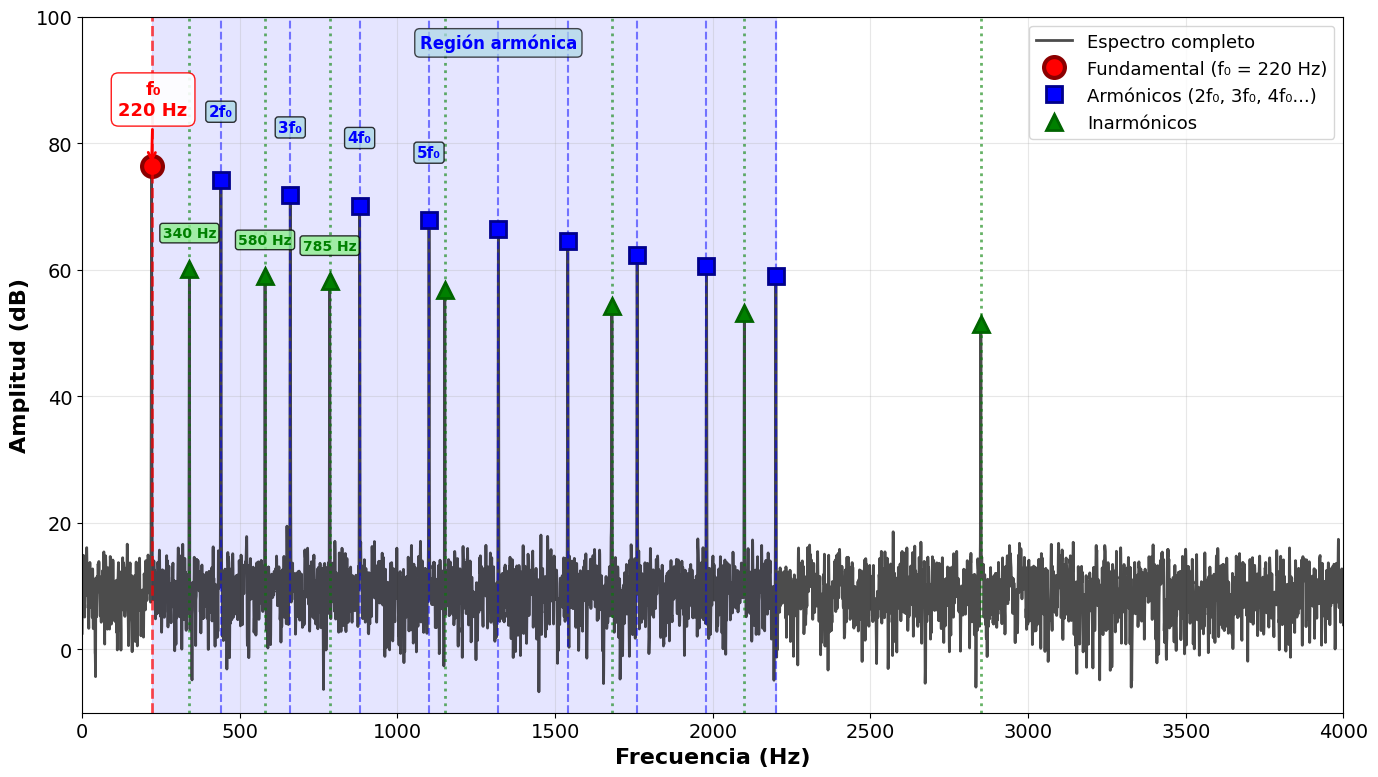
\includegraphics[width=\textwidth]{figures/armonicos.png}
    \caption{Respuesta en frecuencia de una señal marcando su fundamental, armónicos e inarmónicos.}
    \label{armonicos}
\end{figure}

\begin{quote}
    \textbf{Ejemplo clínico.} En un análisis de voz, los armónicos de una vocal ayudan a identificar si un paciente tiene disfonía (por ejemplo, armónicos débiles indican cuerdas vocales dañadas).
\end{quote}

\section{División en bandas y filtros}
Los sonidos se dividen en bandas de frecuencia para analizarlos o modificarlos.

\subsection{Bandas de octava y tercio de octava}
\begin{itemize}
    \item \textbf{Octava:} Una banda donde la frecuencia superior es el doble de la inferior ($f_{\text{sup}} = 2 f_{\text{inf}}$). Por ejemplo, 500–1000 Hz.
    \item \textbf{Tercio de octava:} Banda más estrecha, con factor $\sqrt[3]{2}$ (por ejemplo, 891–1122 Hz para una banda centrada en 1000 Hz).
\end{itemize}

\subsection{Tipos de filtros}
\begin{description}
    \item[\textbf{Pasa bajos (LPF):}] Deja pasar frecuencias bajas, atenúa las altas. Útil para eliminar ruido agudo.
    \item[\textbf{Pasa altos (HPF):}] Deja pasar frecuencias altas, atenúa las bajas. Usado en análisis de consonantes.
    \item[\textbf{Pasa banda (BP):}] Deja pasar un rango específico. Usado en audífonos para amplificar frecuencias perdidas.
    \item[\textbf{Rechaza banda (Notch):}] Elimina un rango estrecho. Útil para reducir acoples en audífonos.
\end{description}

\begin{figure}[h]
    \centering
    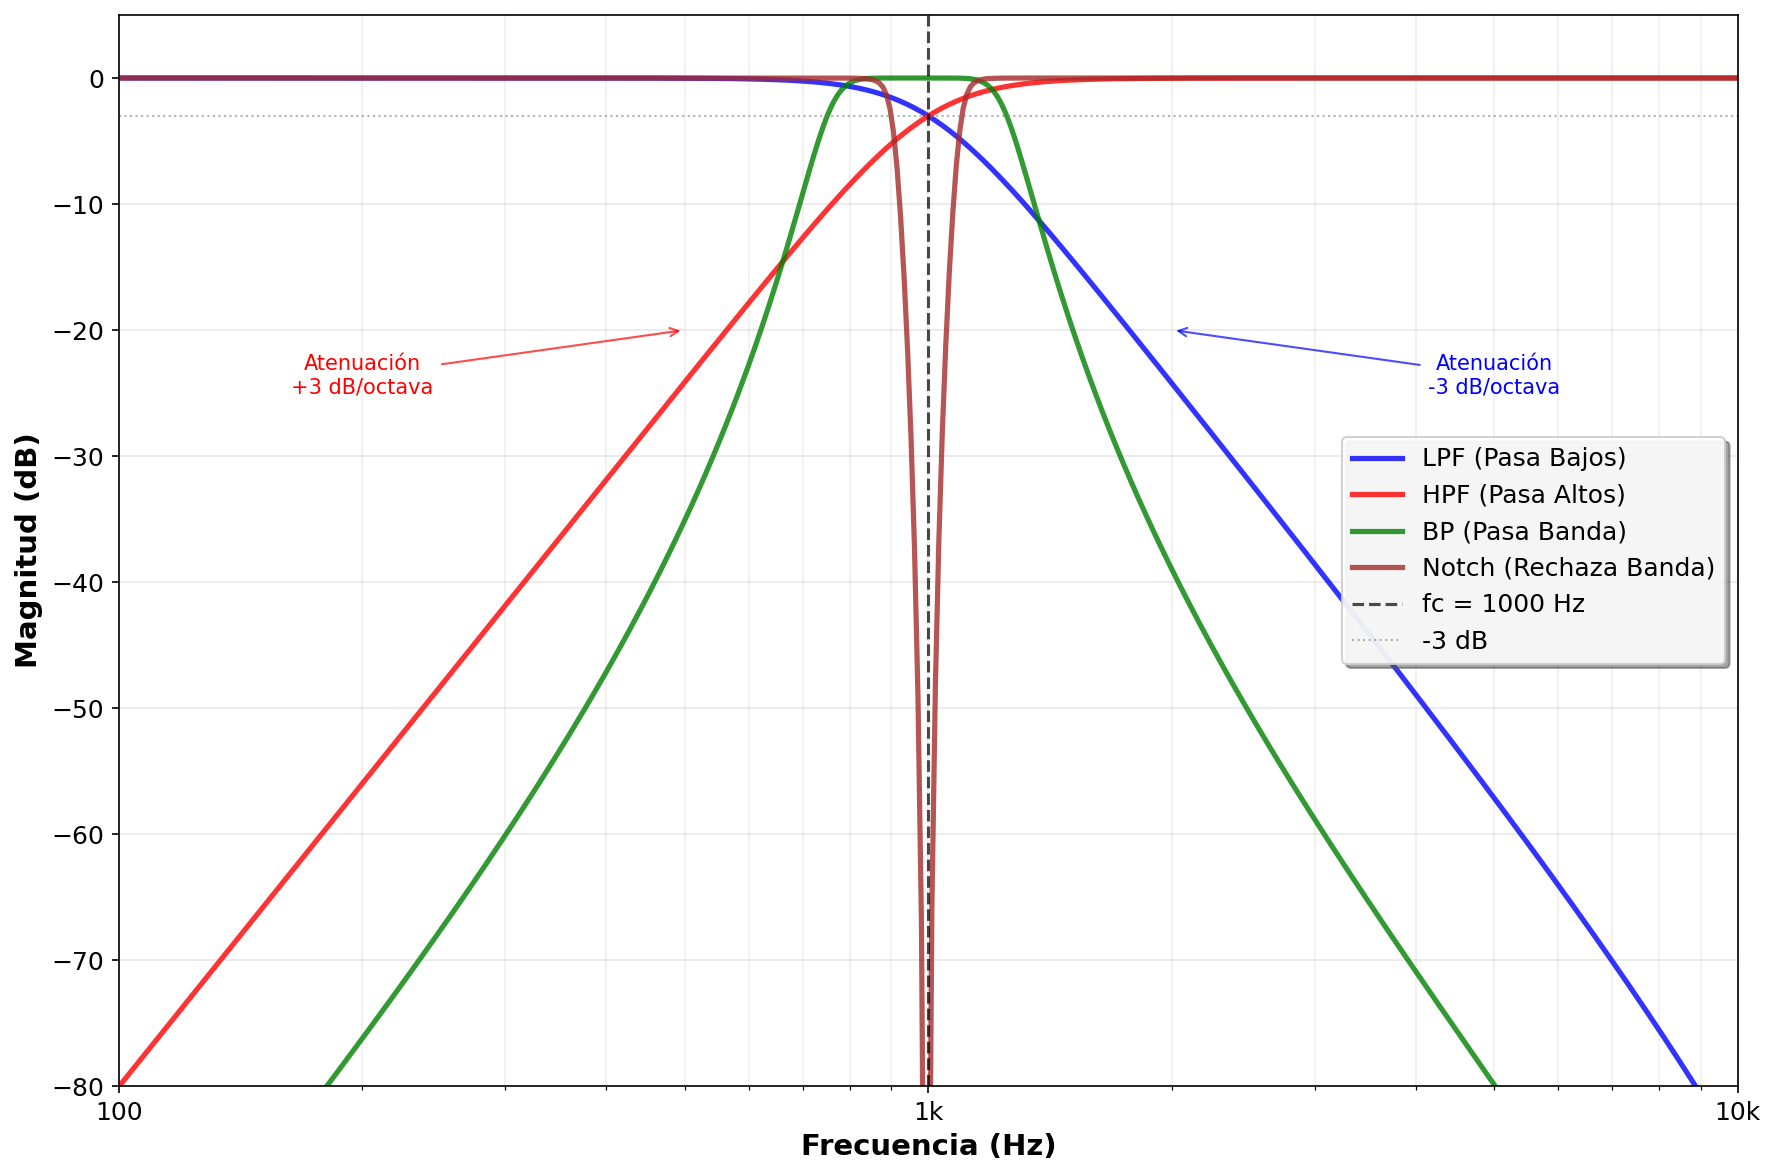
\includegraphics[width=1.0\textwidth]{figures/filtros.png}
    \caption{Diagrama comparativo de filtros LPF, HPF, BP y Notch.}
    \label{filtros}
\end{figure}

\begin{quote}
    \textbf{Ejemplo clínico.} Un audífono usa un filtro pasa banda para amplificar solo las frecuencias donde el paciente tiene pérdida auditiva (por ejemplo, 2000–4000 Hz).
\end{quote}

\textbf{Actividad práctica.} Usa Audacity para aplicar un filtro pasa bajos a una grabación de tu voz (menú ``Efectos'' → ``Filtro''). Nota cómo se eliminan los sonidos agudos (como las ``s'') y compara con un filtro pasa altos.

\section{Curvas de ponderación A, C y Z}
Las curvas de ponderación ajustan las mediciones de sonido según la sensibilidad del oído:
\begin{description}
    \item[\textbf{Curva A:}] Imita la audición a niveles moderados (50–60 dB). Atenúa bajas frecuencias. Usada en normativa de ruido laboral.
    \item[\textbf{Curva C:}] Más plana, mide niveles altos (como en conciertos).
    \item[\textbf{Curva Z:}] Sin ponderación, mide el sonido real.
\end{description}

\begin{table}[h]
    \centering
    \begin{tabular}{|c|c|c|c|}
        \hline
        \textbf{Frecuencia (Hz)} & \textbf{A (dB)} & \textbf{C (dB)} & \textbf{Z (dB)} \\
        \hline
        31.5 & -39.4 & -14.3 & 0 \\
        125 & -16.1 & -3.0 & 0 \\
        1000 & 0.0 & 0.0 & 0 \\
        8000 & +1.0 & -0.2 & 0 \\
        \hline
    \end{tabular}
    \caption{Atenuación aproximada de las curvas de ponderación (IEC 61672).}
\end{table}

\begin{figure}[h]
    \centering
    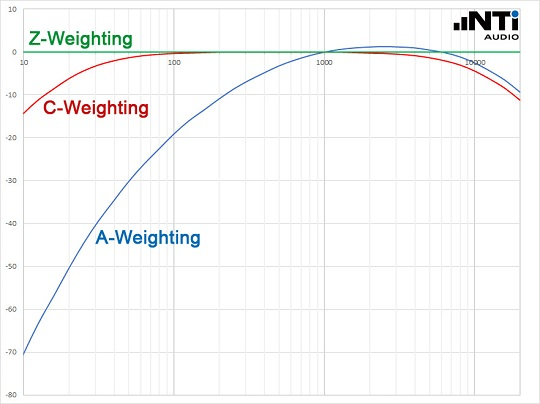
\includegraphics[width=0.8\textwidth]{figures/ponderacion.jpg}
    \caption{Curvas de ponderación A, C y Z.}
    \label{ponderacion}
\end{figure}

Los valores de atenuación para las demás frecuencias se pueden ver en este \href{https://www.nti-audio.com/es/servicio/conocimientos/ponderaciones-de-frecuencia-de-los-niveles-de-sonido}{link}. 

\begin{quote}
    \textbf{Ejemplo clínico.} En una cabina audiométrica, se usa un sonómetro con curva A para asegurar que el ruido de fondo sea < 35 dBA, garantizando pruebas precisas.
\end{quote}

\section{Medidor de nivel de presión sonora (sonómetro)}
Un sonómetro mide el nivel de presión sonora (dBSPL) y puede incluir:
\begin{itemize}
    \item \textbf{Micrófono de campo libre:} Captura el sonido sin reflexiones.
    \item \textbf{Ponderaciones A/C/Z:} Ajusta la medición según el oído humano.
    \item \textbf{Mediciones:} Instantánea (SPL), promedio ($L_{\text{eq}}$), máximo ($L_{\text{max}}$).
\end{itemize}

\begin{quote}
    \textbf{Ejemplo clínico.} Antes de una audiometría, un sonómetro verifica que el ruido en la cabina sea < 35 dBA según ISO 8253-1, asegurando resultados fiables.
\end{quote}

\section{Ejemplos prácticos}
\begin{enumerate}
    \item \textbf{Espectro de una vocal /a/.} Grabada en Audacity, muestra $f_0 = 120$ Hz (pitch), $F_1 = 730$ Hz, $F_2 = 1090$ Hz, $F_3 = 2440$, $F_4 = 3400$ Hz Hz (formantes que dan el timbre).
    \item \textbf{Filtro pasa banda.} Un filtro de 1/3 octava centrado en 1000 Hz (ancho de banda~176 Hz) aplicado a ruido rosa resalta frecuencias del habla.
    \item \textbf{Curva A.} Un tono de 63 Hz medido en 80 dB(Z) se reduce a:
    \[
    L_A = 80 - 26.2 \approx 53.8~\text{dBA}.
    \]
\end{enumerate}

\section{Ejercicios de autoevaluación}
\begin{enumerate}
    \item Usa Audacity para grabar una vocal y observa su espectro. Identifica la frecuencia fundamental ($f_0$) y al menos un formante.
    \item Calcula el nivel resultante de dos fuentes coherentes de 85 dB con diferencia de fase de 90°. (\emph{Pista:} Usa suma de fasores; solución aproximada: 88 dB.)
    \item ¿Qué atenuación aplica la curva A a un tono de 63 Hz? Usa la tabla. (\emph{Solución:} -26.2 dB.)
    \item Explica cómo un filtro pasa banda en un audífono ayuda a un paciente con pérdida auditiva en 2000–4000 Hz.
\end{enumerate}

\section{Recursos recomendados}
\begin{itemize}
    \item Video: \href{https://www.youtube.com/watch?v=r6sGWTCMz2k&ab_channel=3Blue1Brown}{``Qué es una Serie de Fourier? Del Flujo de Calor al Arte con Círculos''.}
    \item Video: \href{https://www.youtube.com/watch?v=spUNpyF58BY&ab_channel=3Blue1Brown}{``Pero, ¿qué es la transformada de Fourier? Una introducción visual.''}
    \item App: Audacity (gratis). Analiza espectros y aplica filtros.
    \item App: Decibel X (gratis). Mide niveles de presión sonora.
    \item Libro: A. Oppenheim, \emph{Signals and Systems}, capítulo 4 (introducción a Fourier).
\end{itemize}

\section*{Glosario}
\begin{description}
    \item[\textbf{FFT:}] Transformada Rápida de Fourier, para analizar frecuencias en señales.
    \item[\textbf{$L_{\text{eq}}$:}] Nivel de presión sonora promedio en un período.
    \item[\textbf{Formante:}] Pico de frecuencia en el espectro de la voz, define el timbre.
    \item[\textbf{Tercio de octava:}] Banda de frecuencia estrecha, usada en análisis acústico.
\end{description}

\section*{Resumen}
\begin{itemize}
    \item \textbf{Fourier:} Descompone señales en frecuencias (fundamental y armónicos), útil para analizar la voz.
    \item \textbf{Rangos de frecuencia:} Audible (20 Hz–20 kHz), infrasonido ($<$20 Hz), ultrasonido ($>$20 kHz).
    \item \textbf{Filtros:} Pasa bajos, pasa altos, pasa banda y Notch, usados en audífonos y análisis.
    \item \textbf{Ponderaciones A/C/Z:} Ajustan mediciones según la audición humana.
\end{itemize}

\bigskip
\noindent\emph{Conclusión.} El análisis frecuencial permite descomponer el sonido en sus componentes, identificar problemas de voz o audición, y diseñar soluciones como audífonos o cabinas audiométricas. Estas herramientas son esenciales para diagnosticar trastornos fonoaudiológicos y garantizar entornos de prueba precisos. En la próxima unidad, exploraremos cómo el cerebro procesa estas señales acústicas.



%%%%%%%%%%%%%%%%%%%%%%%%%%%%%%%%%%%%%%%%%%%%%%%%%%%%%%%%%%%%%%%%%%%%%%%%%%%%%%%%%%%%%%%%%%%%%%%%%%
